% Gráficos do orquestrador dinâmico (líder eleito a cada rodada).
% Pacotes no preâmbulo do documento:
%   \usepackage{pgfplots}
%   \pgfplotsset{compat=1.18}
%
% Mesmas cores das figuras das rodadas de teste fixas. A série adversa
% (mais maliciosos, sem defesa) é sempre vermelha pontilhada com estrela.

\pgfplotsset{
  compat=1.18,
  orquestrador/.style={
    font=\small,
    tick label style={font=\footnotesize},
    label style={font=\small},
    legend style={font=\footnotesize, fill=white, fill opacity=0.9, text opacity=1, draw=black!30},
    line width=0.9pt,
    grid=major,
    major grid style={black!8}
  }
}
\definecolor{serieZero}{RGB}{31,119,180}
\definecolor{serieVinte}{RGB}{44,160,44}
\definecolor{serieCinquenta}{RGB}{230,120,20}
\definecolor{serieSessenta}{RGB}{200,30,30}
\definecolor{serieMaioria}{RGB}{40,40,40}

\begin{figure}[htbp]
  \centering
  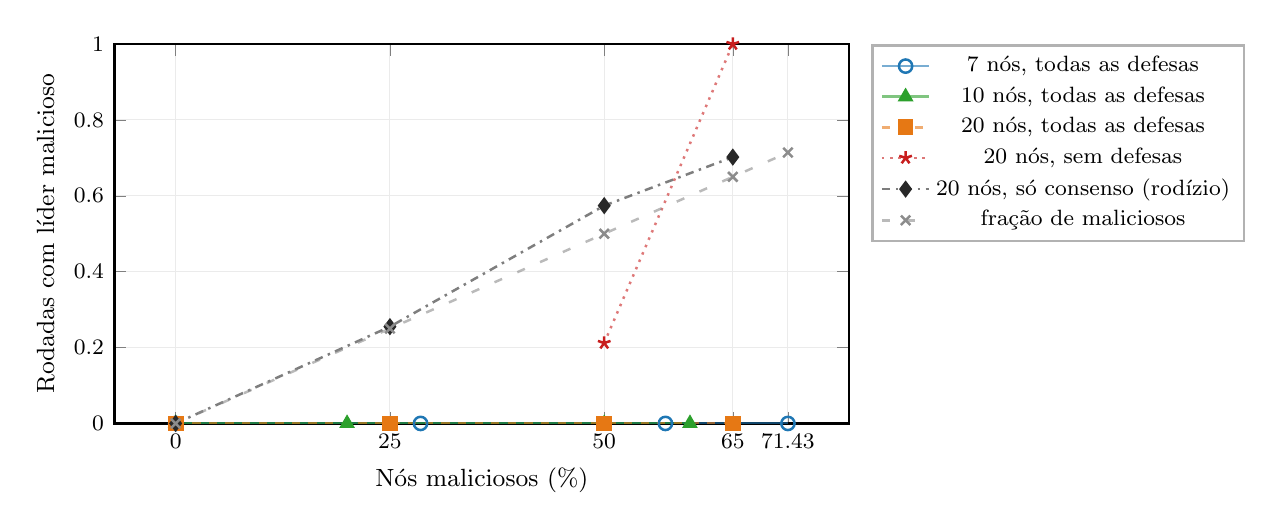
\begin{tikzpicture}
    \begin{axis}[
      orquestrador,
      width=0.9\textwidth,
      height=6.4cm,
      xlabel={Nós maliciosos (\%)},
      ylabel={Rodadas com líder malicioso},
      ymin=0,
      legend pos=outer north east,
      ymax=1,
      xtick={0,25,50,65,71.43}
    ]
\addplot[serieZero, solid, mark=o, opacity=0.6, mark size=2.4pt, mark options={solid, opacity=1}] coordinates {(0,0.000) (28.57,0.000) (57.14,0.000) (71.43,0.000)};
\addlegendentry{7 nós, todas as defesas}
\addplot[serieVinte, solid, mark=triangle*, opacity=0.6, mark size=2.4pt, mark options={solid, opacity=1}] coordinates {(0,0.000) (20,0.000) (50,0.000) (60,0.000)};
\addlegendentry{10 nós, todas as defesas}
\addplot[serieCinquenta, dashed, mark=square*, opacity=0.6, mark size=2.4pt, mark options={solid, opacity=1}] coordinates {(0,0.000) (25,0.000) (50,0.000) (65,0.000)};
\addlegendentry{20 nós, todas as defesas}
\addplot[serieSessenta, dotted, mark=star, opacity=0.6, mark size=2.4pt, mark options={solid, opacity=1}] coordinates {(50,0.212) (65,1.000)};
\addlegendentry{20 nós, sem defesas}
\addplot[serieMaioria, dashdotted, mark=diamond*, opacity=0.6, mark size=2.4pt, mark options={solid, opacity=1}] coordinates {(0,0.000) (25,0.255) (50,0.574) (65,0.702)};
\addlegendentry{20 nós, só consenso (rodízio)}
\addplot[black!45, loosely dashed, mark=x, opacity=0.6, mark size=2.4pt, mark options={solid, opacity=1}] coordinates {(0,0.000) (25,0.250) (50,0.500) (65,0.650) (71.43,0.714)};
\addlegendentry{fração de maliciosos}
    \end{axis}
  \end{tikzpicture}
  \caption{Fração das rodadas, depois da calibração, em que o líder eleito é malicioso. Grafo 4-regular, líder que forja, sinal híbrido (exceto a série de consenso puro, em que o poder de voto não se separa e a eleição vira rodízio). Média entre repetições e mecanismos. A linha de referência é a fração de nós maliciosos na rede.}
  \label{fig:dinamico-lideranca}
\end{figure}

\begin{figure}[htbp]
  \centering
  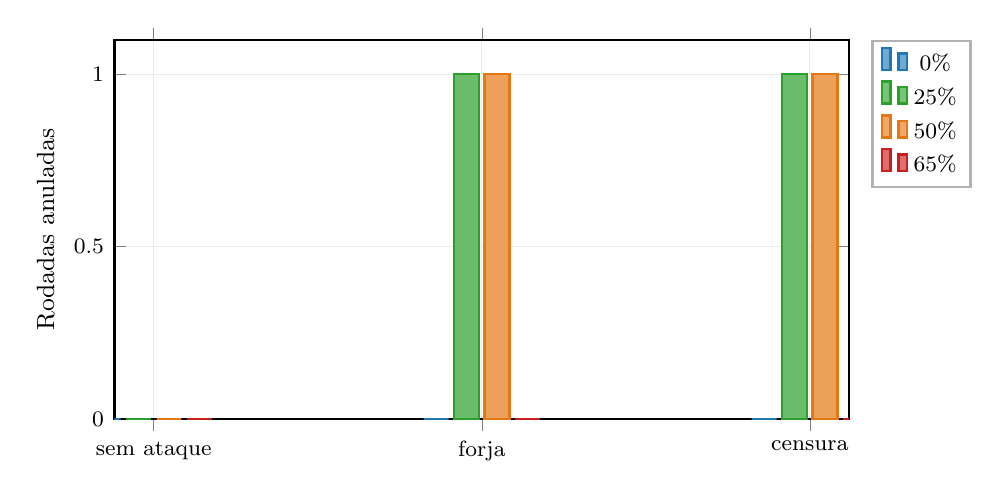
\begin{tikzpicture}
    \begin{axis}[
      orquestrador,
      ybar,
      symbolic x coords={none,forge,censor},
      xtick=data,
      xticklabels={{sem ataque},{forja},{censura}},
      width=0.9\textwidth,
      height=6.4cm,
      ylabel={Rodadas anuladas},
      ymin=0,
      bar width=9pt,
      legend pos=outer north east,
      enlarge x limits=0.06
    ]
\addplot[fill=serieZero!70, draw=serieZero] coordinates {(none,0.000) (forge,0.000) (censor,0.000)};
\addlegendentry{0\%}
\addplot[fill=serieVinte!70, draw=serieVinte] coordinates {(none,0.000) (forge,1.000) (censor,1.000)};
\addlegendentry{25\%}
\addplot[fill=serieCinquenta!70, draw=serieCinquenta] coordinates {(none,0.000) (forge,1.000) (censor,1.000)};
\addlegendentry{50\%}
\addplot[fill=serieSessenta!70, draw=serieSessenta] coordinates {(none,0.000) (forge,0.000) (censor,0.000)};
\addlegendentry{65\%}
    \end{axis}
  \end{tikzpicture}
  \caption{Rodadas anuladas (de 50) por tipo de ataque do líder, 20 nós, todas as defesas. Média entre repetições e mecanismos. A forja ou a censura só derruba a rodada do líder malicioso.}
  \label{fig:dinamico-anuladas}
\end{figure}

\begin{figure}[htbp]
  \centering
  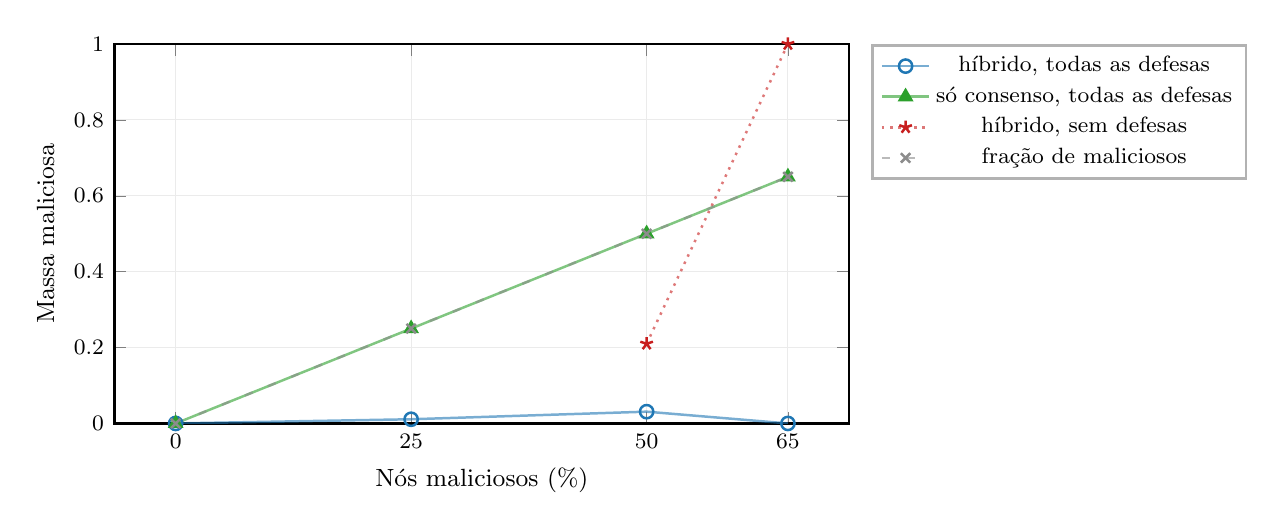
\begin{tikzpicture}
    \begin{axis}[
      orquestrador,
      width=0.9\textwidth,
      height=6.4cm,
      xlabel={Nós maliciosos (\%)},
      ylabel={Massa maliciosa},
      ymin=0,
      legend pos=outer north east,
      ymax=1,
      xtick={0,25,50,65}
    ]
\addplot[serieZero, solid, mark=o, opacity=0.6, mark size=2.4pt, mark options={solid, opacity=1}] coordinates {(0,0.000) (25,0.011) (50,0.031) (65,0.000)};
\addlegendentry{híbrido, todas as defesas}
\addplot[serieVinte, solid, mark=triangle*, opacity=0.6, mark size=2.4pt, mark options={solid, opacity=1}] coordinates {(0,0.000) (25,0.250) (50,0.500) (65,0.650)};
\addlegendentry{só consenso, todas as defesas}
\addplot[serieSessenta, dotted, mark=star, opacity=0.6, mark size=2.4pt, mark options={solid, opacity=1}] coordinates {(50,0.210) (65,1.000)};
\addlegendentry{híbrido, sem defesas}
\addplot[black!45, loosely dashed, mark=x, opacity=0.6, mark size=2.4pt, mark options={solid, opacity=1}] coordinates {(0,0.000) (25,0.250) (50,0.500) (65,0.650)};
\addlegendentry{fração de maliciosos}
    \end{axis}
  \end{tikzpicture}
  \caption{Massa de reputação dos maliciosos ao fim de 50 rodadas, na cópia da cadeia seguida pela maioria dos honestos, 20 nós, líder que forja. Acima de 0,5 o conluio fecha o quórum sozinho.}
  \label{fig:dinamico-massa}
\end{figure}

\begin{figure}[htbp]
  \centering
  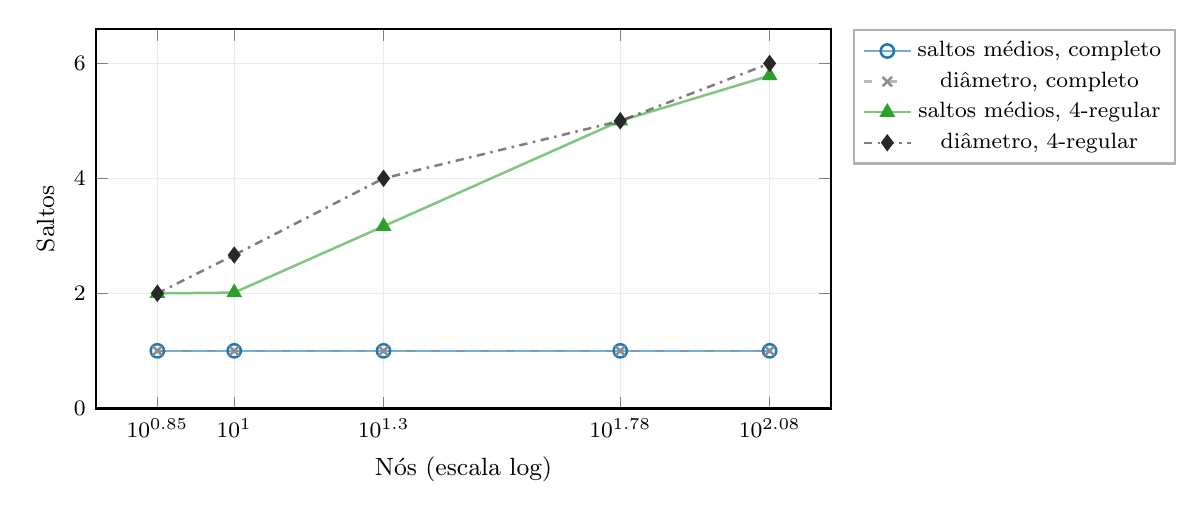
\begin{tikzpicture}
    \begin{axis}[
      orquestrador,
      width=0.9\textwidth,
      height=6.4cm,
      xlabel={Nós (escala log)},
      ylabel={Saltos},
      ymin=0,
      legend pos=outer north east,
      xtick={7,10,20,60,120},
      xmode=log
    ]
\addplot[serieZero, solid, mark=o, opacity=0.6, mark size=2.4pt, mark options={solid, opacity=1}] coordinates {(7,1.000) (10,1.000) (20,1.000) (60,1.000) (120,1.000)};
\addlegendentry{saltos médios, completo}
\addplot[black!45, loosely dashed, mark=x, opacity=0.6, mark size=2.4pt, mark options={solid, opacity=1}] coordinates {(7,1.000) (10,1.000) (20,1.000) (60,1.000) (120,1.000)};
\addlegendentry{diâmetro, completo}
\addplot[serieVinte, solid, mark=triangle*, opacity=0.6, mark size=2.4pt, mark options={solid, opacity=1}] coordinates {(7,2.000) (10,2.013) (20,3.167) (60,5.000) (120,5.787)};
\addlegendentry{saltos médios, 4-regular}
\addplot[serieMaioria, dashdotted, mark=diamond*, opacity=0.6, mark size=2.4pt, mark options={solid, opacity=1}] coordinates {(7,2.000) (10,2.667) (20,4.000) (60,5.000) (120,6.000)};
\addlegendentry{diâmetro, 4-regular}
    \end{axis}
  \end{tikzpicture}
  \caption{Saltos da difusão da tarefa (do líder ao nó mais distante) por tamanho da rede, 25\% de maliciosos sem conluio. No grafo completo cada nó mantém N-1 conexões; no 4-regular, 4.}
  \label{fig:dinamico-saltos}
\end{figure}

\begin{figure}[htbp]
  \centering
  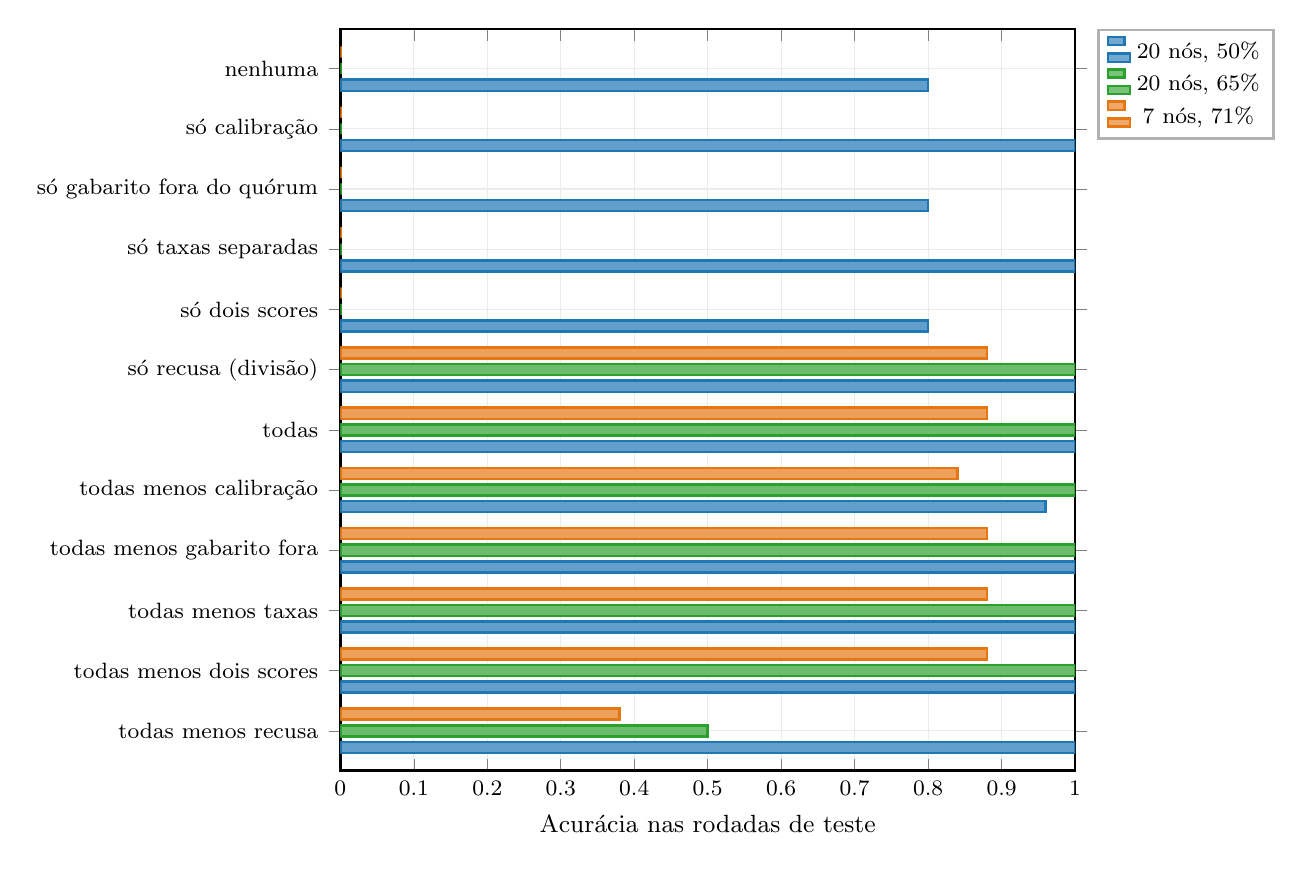
\begin{tikzpicture}
    \begin{axis}[
      orquestrador,
      xbar,
      symbolic y coords={allminusrefuseforged,allminussplitscores,allminussplitalpha,allminusoraclebypass,allminuscalibration,all,refuseforged,splitscores,splitalpha,oraclebypass,calibration,none},
      ytick=data,
      yticklabels={{todas menos recusa},{todas menos dois scores},{todas menos taxas},{todas menos gabarito fora},{todas menos calibração},{todas},{só recusa (divisão)},{só dois scores},{só taxas separadas},{só gabarito fora do quórum},{só calibração},{nenhuma}},
      width=0.9\textwidth,
      height=11cm,
      xlabel={Acurácia nas rodadas de teste},
      xmin=0,
      bar width=4pt,
      legend pos=outer north east,
      enlarge y limits=0.06,
      xmax=1
    ]
\addplot[fill=serieZero!70, draw=serieZero] coordinates {(1.000,allminusrefuseforged) (1.000,allminussplitscores) (1.000,allminussplitalpha) (1.000,allminusoraclebypass) (0.960,allminuscalibration) (1.000,all) (1.000,refuseforged) (0.800,splitscores) (1.000,splitalpha) (0.800,oraclebypass) (1.000,calibration) (0.800,none)};
\addlegendentry{20 nós, 50\%}
\addplot[fill=serieVinte!70, draw=serieVinte] coordinates {(0.500,allminusrefuseforged) (1.000,allminussplitscores) (1.000,allminussplitalpha) (1.000,allminusoraclebypass) (1.000,allminuscalibration) (1.000,all) (1.000,refuseforged) (0.000,splitscores) (0.000,splitalpha) (0.000,oraclebypass) (0.000,calibration) (0.000,none)};
\addlegendentry{20 nós, 65\%}
\addplot[fill=serieCinquenta!70, draw=serieCinquenta] coordinates {(0.380,allminusrefuseforged) (0.880,allminussplitscores) (0.880,allminussplitalpha) (0.880,allminusoraclebypass) (0.840,allminuscalibration) (0.880,all) (0.880,refuseforged) (0.000,splitscores) (0.000,splitalpha) (0.000,oraclebypass) (0.000,calibration) (0.000,none)};
\addlegendentry{7 nós, 71\%}
    \end{axis}
  \end{tikzpicture}
  \caption{Ablação das defesas contra conluio: acurácia do consenso ponderado nas rodadas de teste, líder que forja. Média entre repetições e mecanismos.}
  \label{fig:dinamico-ablacao}
\end{figure}
